\documentclass[tikz,border=3pt]{standalone}
\usepackage[T1]{fontenc}
\usepackage{mathptmx}
\usepackage{tikz,pgfplots}
\usetikzlibrary{arrows.meta,positioning,calc,fit,backgrounds,shapes.geometric}
\pgfplotsset{compat=1.18}
\definecolor{forest}{HTML}{346E57}
\definecolor{sage}{HTML}{E8EFEA}
\definecolor{clay}{HTML}{AC653F}
\definecolor{sand}{HTML}{F4EAE2}
\definecolor{ink}{HTML}{252525}
\definecolor{light}{HTML}{F5F5F3}
\definecolor{gridgray}{HTML}{D8DAD6}
\tikzset{box/.style={draw=ink!70,line width=.5pt,rectangle,rounded corners=1pt,fill=white,align=center,font=\fontsize{11}{12}\selectfont,inner sep=6pt}, flow/.style={-{Latex[length=2.4mm]},line width=.7pt,draw=ink!80}, data/.style={flow,densely dashed,draw=forest}, label/.style={font=\fontsize{10}{11}\selectfont,fill=white,inner sep=2pt,align=center}}
\hyphenpenalty=10000\exhyphenpenalty=10000\begin{document}
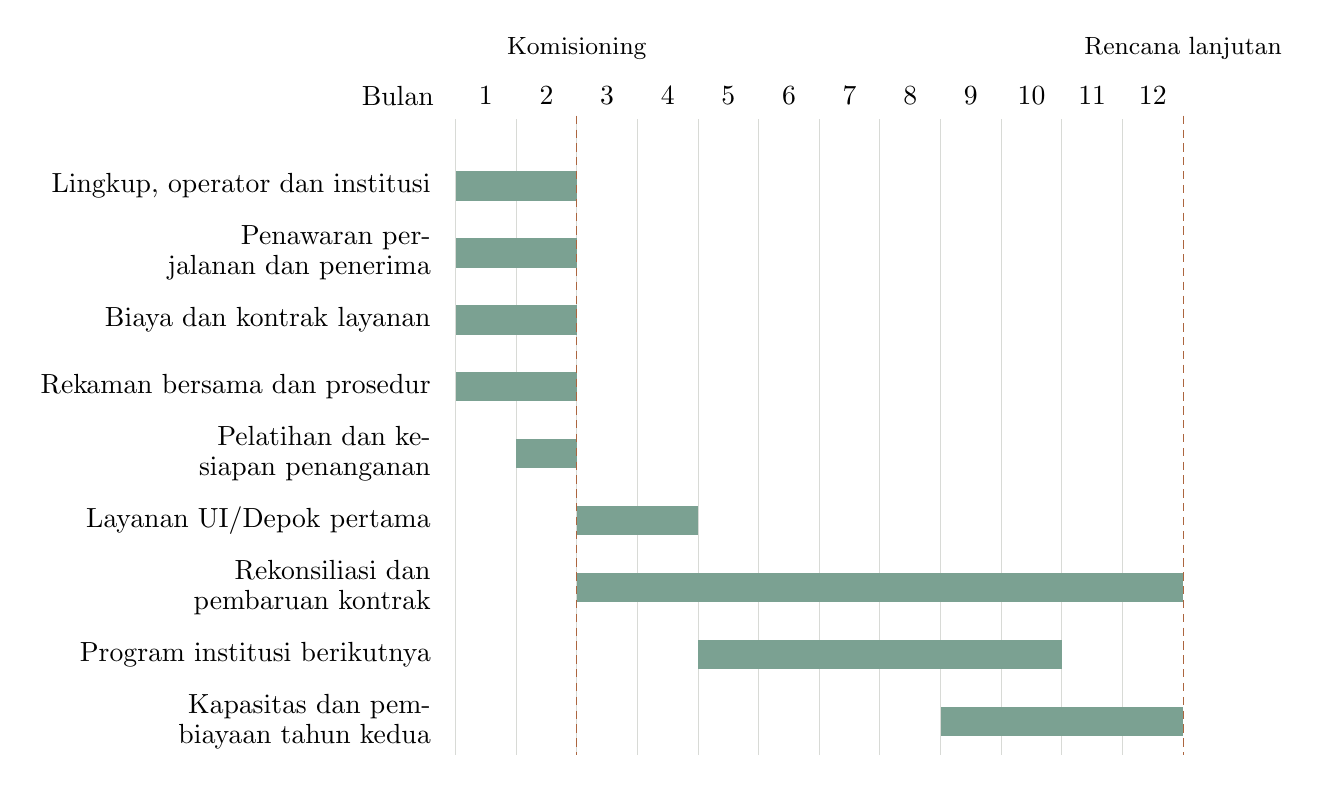
\begin{tikzpicture}[x=.77cm,y=.85cm]
\def\rows{9}
\foreach\m in{1,...,12}{\draw[gridgray,line width=.35pt](\m,0)--(\m,-9.5);\node[font=\fontsize{10}{11}\selectfont]at(\m+.5,.35){\m};}
\node[anchor=east,font=\fontsize{10}{11}\selectfont]at(.8,.35){Bulan};
\foreach\y/\s/\e/\lab in {1/1/2/{Lingkup, operator dan institusi},2/1/2/{Penawaran perjalanan dan penerima},3/1/2/{Biaya dan kontrak layanan},4/1/2/{Rekaman bersama dan prosedur},5/2/2/{Pelatihan dan kesiapan penanganan},6/3/4/{Layanan UI/Depok pertama},7/3/12/{Rekonsiliasi dan pembaruan kontrak},8/5/10/{Program institusi berikutnya},9/9/12/{Kapasitas dan pembiayaan tahun kedua}}{
\node[anchor=east,text width=5cm,align=right,font=\fontsize{10}{11}\selectfont]at(.75,-\y){\lab};\fill[forest!65](\s,-\y-.22)rectangle(\e+1,-\y+.22);}
\foreach\x/\lab in{3/{Komisioning},13/{Rencana lanjutan}}{\draw[clay,densely dashed](\x,.05)--(\x,-9.5);\node[anchor=south,rotate=0,font=\fontsize{9}{10}\selectfont,text=black]at(\x,.75){\lab};}
\end{tikzpicture}
\end{document}
